\subsubsection{2001: Gerhard Fischer}
\label{sec:fischer_user_2001}

In 2001~\citet{fischer_user_2001} reviews the user models of the past 10 years. 
He describes how using computers in \ac{hci} environments has been always
modelled as a user-computer couple. These elements are modelled as an explicit 
connection which represents the communication between them. New and modern 
interfaces such as windows, menus, pointers, colours, sound and touch screens 
have enlarged this communication line thanks to their capabilities.

Furthermore, in addition to the possibilities of new design approaches,
knowledge-based architectures in \ac{hci} explore the possibility of implicit
communication channel. The required knowledge considers the problem domain,
communication processes and the communication agent. Users are part of the
communication agent group. Fischer defends the idea that there are many types of
users. Besides, their needs change with the experience and through time.
Hence, a simple user classifications (e.g., \textit{novel}, \textit{intermediate}
and \textit{expert}) is not enough to characterize users in complex environments. 
Nevertheless, despite Fischer remarks the significance of each agent, he does 
not establish which agent capabilities are important to face the problem of 
modelling a user.

% \InsertFig{fischer}{fig:fischer}{The human-computer interaction channel 
% \citep{fischer_user_2001}}{}{0.70}{}

\begin{figure}
\centering
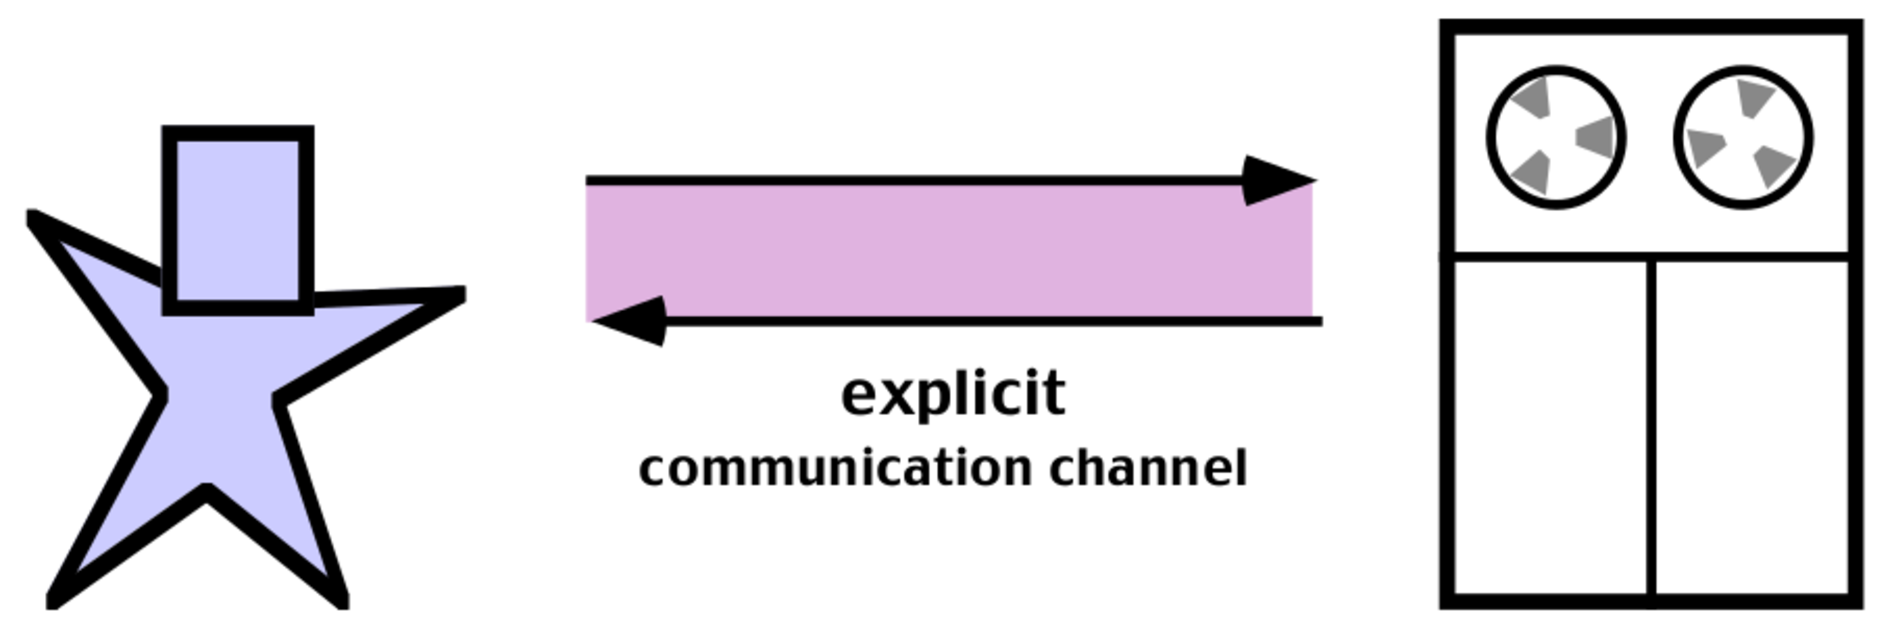
\includegraphics[width=0.50\textwidth]{fischer.pdf}
\caption{The \ac{hci} channel~\citep{fischer_user_2001}.}
\label{fig:fischer}
\end{figure}